%pdflatex-../thesis.tex
% vim:spell spelllang=en_us

% introduction to models
Purpose of the cloud computing is to deliver the service and provide customers with tools to manage this service. Service models differs by level of control provided to customers and thus with areas of responsibility. I am going to call border between responsibility of customer and responsibility of provider as responsibility border. Responsibility borders according to service models are depicted in the figure \ref{img:service-models}.

Some of the service models leave almost all control and responsibility at provider's side and other supplies customer with more control. It is necessary to select right service model according to expected service usage and required control level.

\subsection{Infrastructure as a Service}
\Ac{IaaS} is a model with the most of a configuration tasks left at customer's side. Customer is responsible for the virtual machines and it's services, so it gives much more flexibility than other models and it is well-suited for services with extraordinary requirements. 

Customer manages virtual machines as well as running services, so provider is responsible only for the virtualization and underneath layers. It is even possible to run custom operating system, but provider usually offers prepared images. Prepared \Ac{OS} images are tested and modified to run well in cloud environment. There can be preinstalled hybrid virtualization drivers, kernel tweaked to run virtualized and it is also good idea to remove unused drivers and software. 

This model is good choice if special configuration is needed, but service deployment is more difficult because some expertise is needed. \Ac{IaaS} can be used if customer require additional level of security because virtual machine can use crypted volume and make disk unreadable for provider. Unfortunately it is still possible for provider to acquire confidential from other sources, for example from memory, but it is much more complicated.

Typical example of \Ac{IaaS} is Amazon Web Services and Active24's VPS.

\subsection{Platform as a Service}
Border of responsibility of \Ac{PaaS} is located two layers higher compared to \Ac{IaaS}. Service provider is responsible for platform and all underlaying layers, thus provider takes care of same layers as in \Ac{IaaS} plus operating system and platform. 
Leaving operating system maintenance on provider's side may be beneficial because provider can adjust operating system for virtualization and takes care about software updates. 

Provider usually manages a many operating systems for many customers, so the updating and maintenance tasks may be automatized or executed in a batch. Sharing the operating system layer between customers with preserving adequate level of isolation can save many resource and make operating system administration easier.

Customer using service according to this model runs his own software and does not take care of any lower layers. It is not necessary to do any administration tasks and more effort can be given to application development. 

This model is well-suited for running applications without any special requirements. It makes service deployment faster and easier, but is more limited by used platform. 
Typical example is project Evia and Microsoft Azure.

\subsection{Software as a Service}
\Ac{SaaS} is model with none of the administration tasks left at customer's responsibility. Software is hosted and maintained by service provider and customer is using the service. Service is accessed remotely via network (usually the Internet). It is common mistake to say, that service is accessed as Web service because any remote access can be used. 

This model is right solution for customers looking for service without hassling with it's administration.

\begin{figure}[htb]
	\begin{center}
	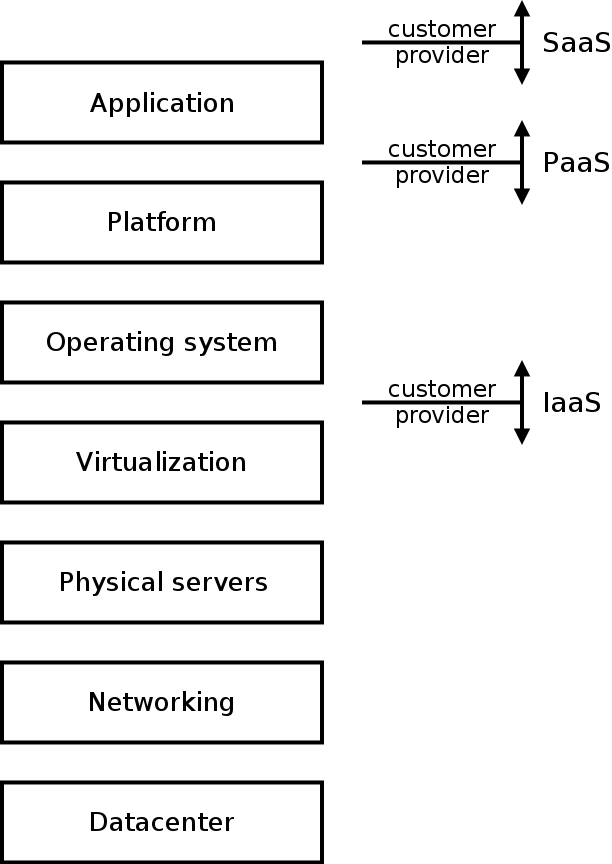
\includegraphics[width=0.5\textwidth]{service-models.png}
	\end{center}
	\caption{Service model responsibility}
	\label{img:service-models}
\end{figure}

